The electronic system used in TRITIUM-Aveiro 0 prototype consists of several PCB and can be divided into two parts:
\begin{enumerate}
\item{} A PCB, whose electronic scheme is shown in Figure \ref{fig:HVElectronicAveiro}, was designed to power the PMTs with a negative high voltage. It consists of several high voltage power supply, model C11152-01 from Hamamatsu company \cite{PowerSupplyAveiroDataSheet}, one for each PMT used, which is controled by a DAC\footnote{DAC, Digital-to-analog converter}, model MAX5500 from Maxim Integrated company \cite{MAX5500DataSheet}. An Arduino Mega is used for the DAC communication and cross-checking the output values and it is connected to a Raspberry Pi to control the system.

A graphical interface, shown Figure \ref{subfig:GUI}, has been developed to manage the different options of this system in a comfortable way.

\begin{figure}
\centering
    \begin{subfigure}[b]{0.45\textwidth}
    \centering
    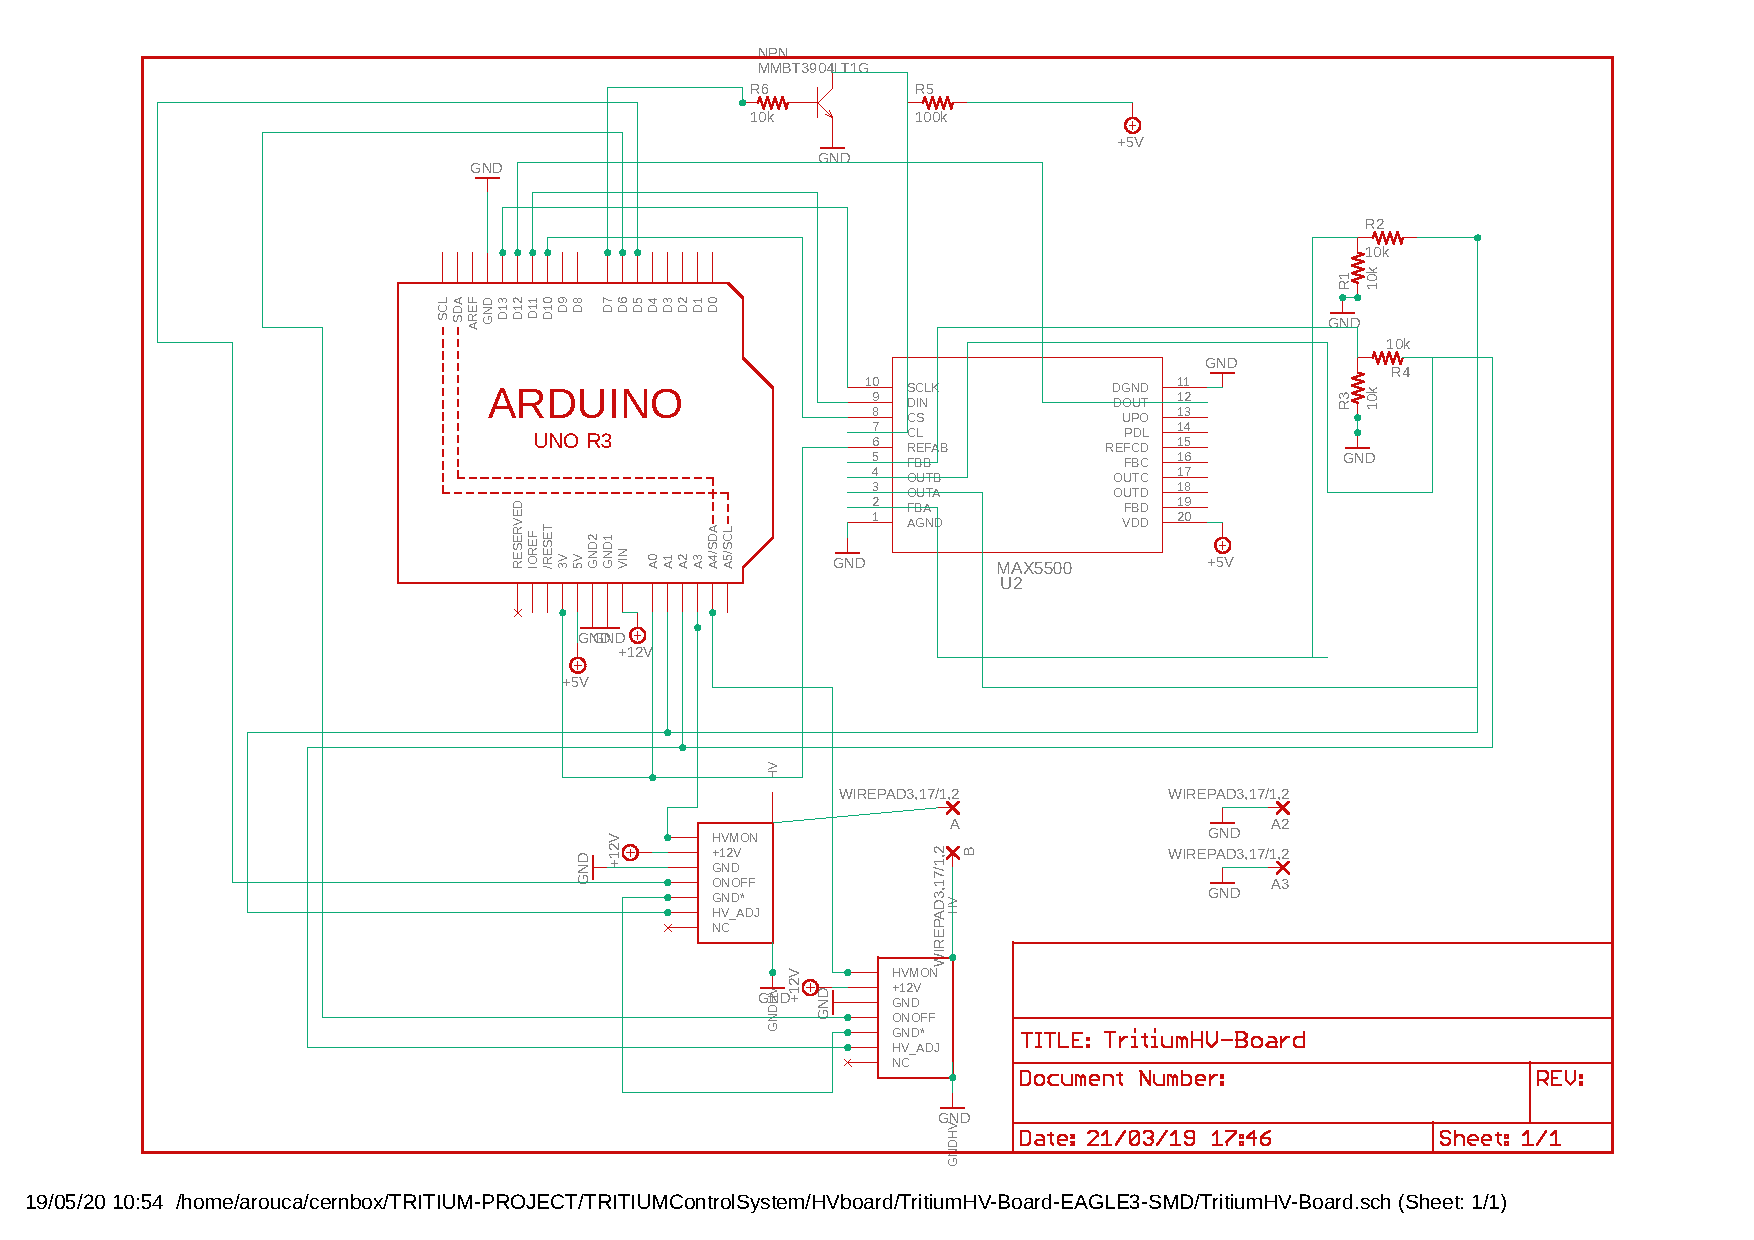
\includegraphics[width=\textwidth]{5Prototypes/53FinalPrototypes/531TritiumAveiro/TritiumHV-Board.pdf}  
    \caption{Electronic scheme of the PCB.\label{subfig:ElectronicSchemeHVBoard}}
    \end{subfigure}
    \hfill
    \begin{subfigure}[b]{0.45\textwidth}
    \centering
    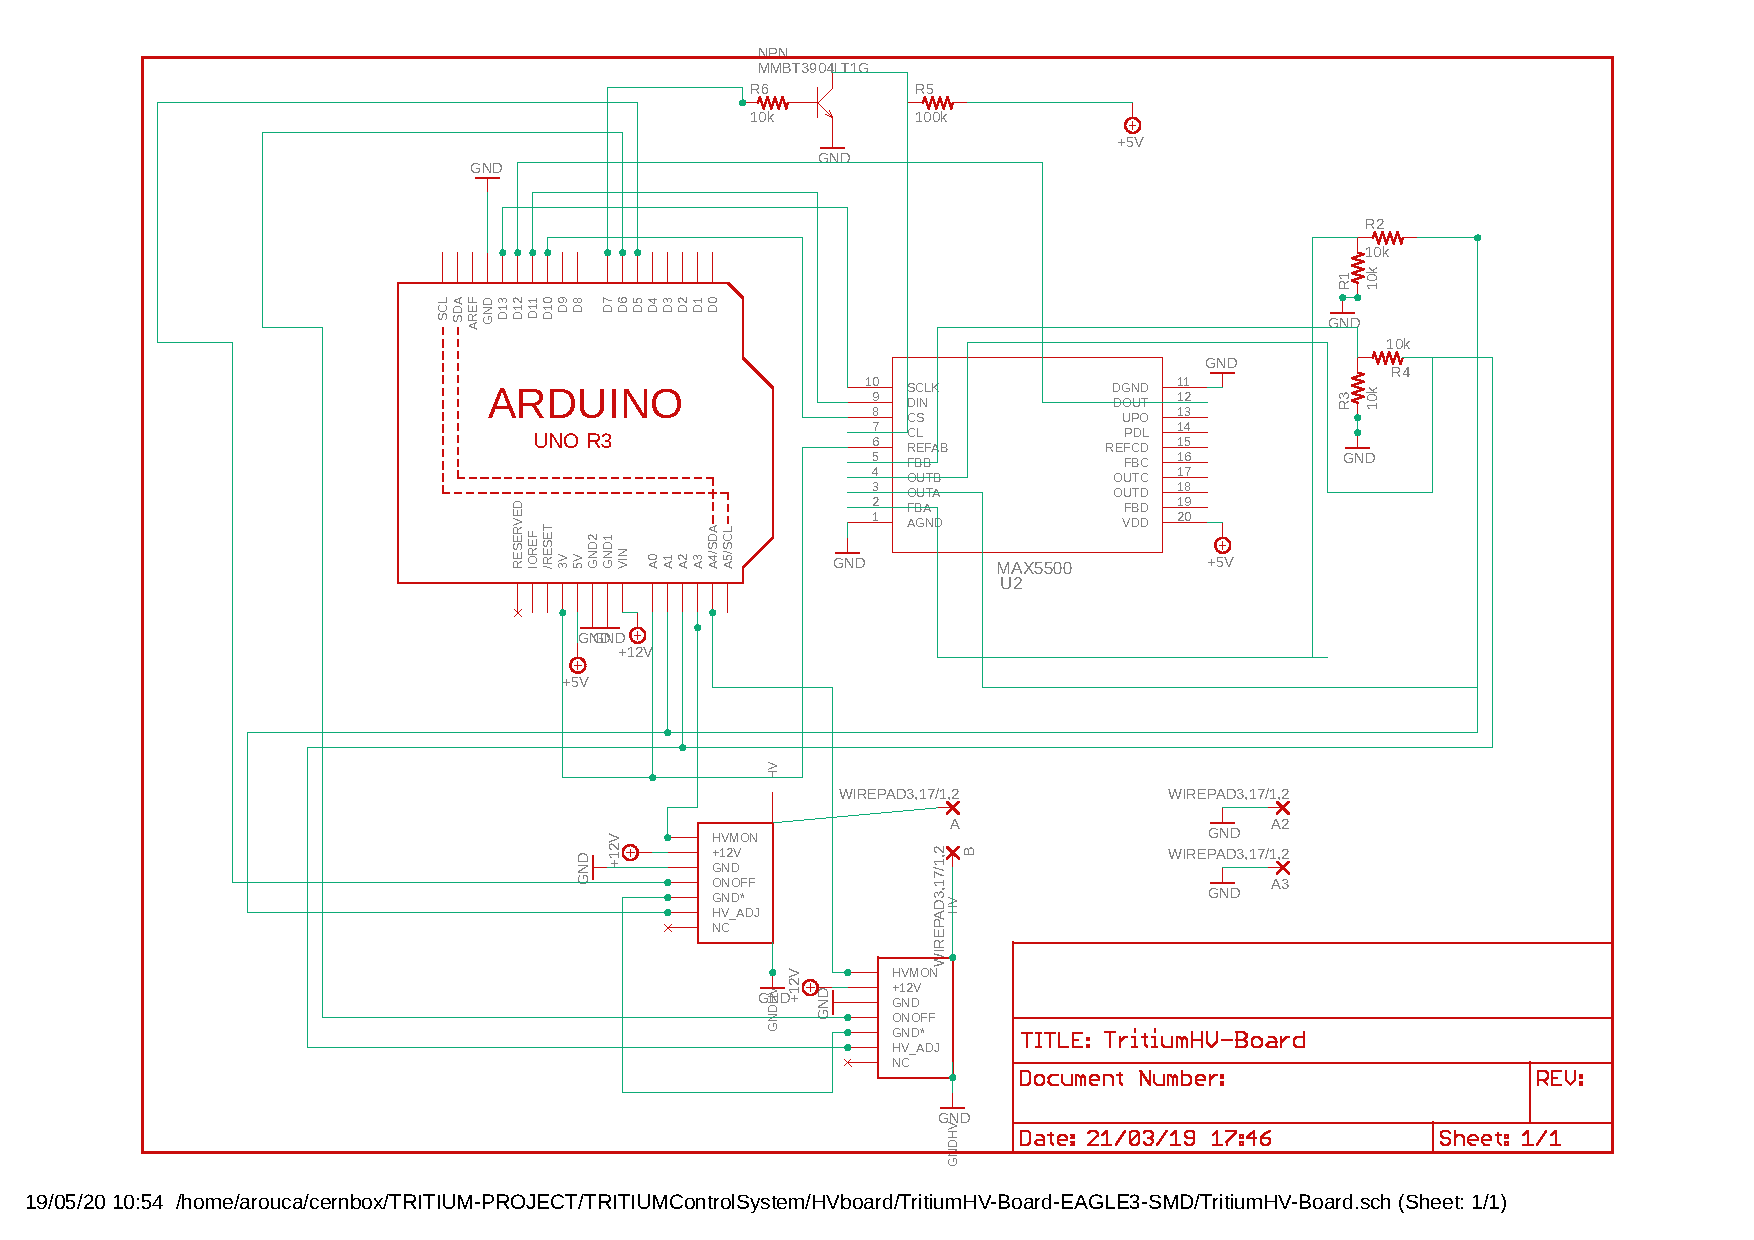
\includegraphics[width=\textwidth]{5Prototypes/53FinalPrototypes/531TritiumAveiro/TritiumHV-Board.pdf}  
    \caption{Graphical user interface.\label{subfig:GUI}}
    \end{subfigure}
 \caption{Electronic scheme of the PCB designed to power the PMTs of Aveiro prototype and the graphical user interface developed to control it.}
 \label{fig:HVElectronicAveiro}
\end{figure}

\item{} A electronical chain consisting of several PCBs was used to process and analyze the system signals, whose simplified electronic scheme is shown in Figure \ref{fig:ElectronicSchemCounterBoard}.

\begin{figure}[h]
\centering
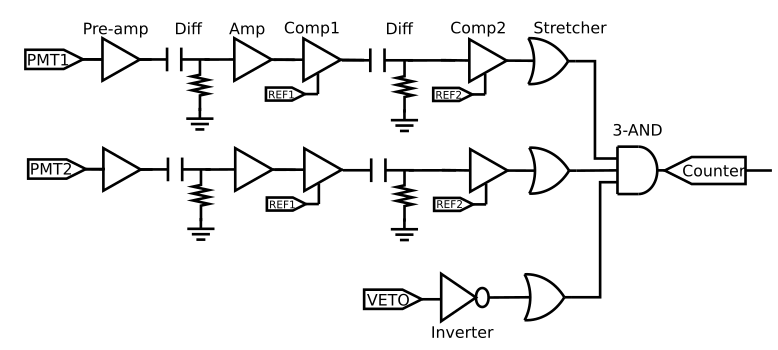
\includegraphics[scale=0.45]{5Prototypes/53FinalPrototypes/531TritiumAveiro/ElectronicSchemeCounterBoard.png}
\caption{Simplified electronic scheme used to process and analyze the signal of TRITIUM-Aveiro 0 prototype. \label{fig:ElectronicSchemCounterBoard}}
\end{figure}

It consists of three different lines, two of them are used for the PMT signals of the prototype and the remaining line is used for doing anticoincidence with a active veto.

To test this electronic chain a plastic scintillation with dimensions of $10 \cdot{} 10 \cdot{} 1~\cm^3$ was used to simulate a veto signal but four different vetos are being developed, each one is based on a rectangular plastic scintillations of Saint-Gobain company \cite{VetoAveiro}, whose dimensiones are $50~\cm \cdot{} 30 \cdot{} 2~\cm^3$  with a PMT coupled, model R2154-02 2" from Hamamatsu company \cite{DataSheetPMTsAveiro}. The output signal of these PMTs will be input in a OR stage, whose response will be introduced in the veto line shown previously in Figure \ref{fig:ElectronicSchemCounterBoard}. As a result, each plastic scintillator will be read in anticoincidence with tritium-Aveiro prototype.

Both lines, used to process and analyze the PMT signals of the prototype, are equal and they are used to operate in time coincidence. First, each PMT signal is introduced in a prepamplifier model CR111 from CREMAT Inc. company \cite{CREMATPreAmplifierDataSheet}, which is used to shape and pre-amplify the signal. To reduce electronic noise and signal loss, both preamplifiers are connected as close as possible to the PMTs and they are located inside of aluminum boxes which act like a Faraday cage.

Each preamplifier is followed by a differentiation stage, which is used to reduce the time width of the signal, and amplification stages, used to amplify the signal. The amplification used is the model OPA656 from Texas Instruments \cite{OPA656}. 

Then, a fast comparator, model LT111 from Linear Technology company \cite{LT111}, is used to set a threshold which will be used to remove the PMT signals whose amplitude are below this value (dark counts of the PMT). A MAX5500 DAC is used to configure the thresholds.

The time width of the preamplfier output signal is too large, $200~\mu\second$, so which too many false coincidence will be registed. To solve this problem a second differenciation stage is included and a second comparator are added to produce a 5V square signal again.

Finally a tunable pulse stretcher based on an OR gate, model SN74AHC1 from Texas Instruments company \cite{Stretcher}, is used to set the time width of each signal at $100~\nano\second$, with which the time coincidence windows of our adquisition system is $200~\nano\second$, narrow enough to have a negligible false coincidence rate.

In the remaining line, used for the veto signal, an inverter is used in the first stage. With it, the signal will always be in the high level, $5~\volt$, except when a cosmic particle is detected, in which case the signal will be in the low level, $0~\volt$. Then, another stretcher is used to create a signal with the same time width than the others, $100~\nano\second$.

Lastly, these three signals are introduced into a 3-input AND gate, model SN74LVC1G11 from Texas Instruments company \cite{ANDGate}, to perform a logic level comparison. With this last stage we achieve a temporal coincidence of both PMT signals of the prototype and anti-coincidence of them with the veto signal. The output signal of this last stage is simply connected to a pulse counter. 

A GPIO pins of a Raspberry Pi is used to communication with the system, control it and configure the different threshold levels and a graphical user interface, whose appearance is shown in Figure \ref{fig:GUIcounts}, has been developed to manage in a comfortable way the counter system.

 \begin{figure}[h]
\centering
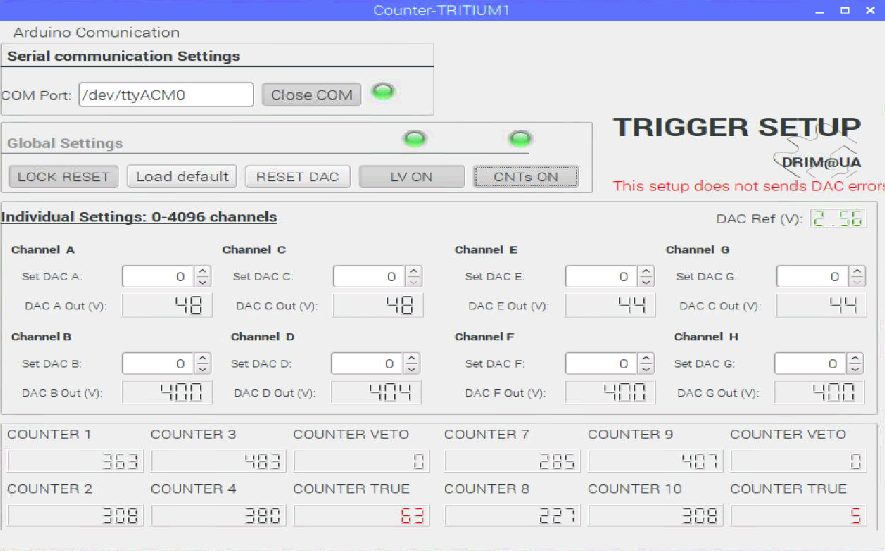
\includegraphics[scale=0.45]{5Prototypes/53FinalPrototypes/531TritiumAveiro/CounterGUI.png}
\caption{Graphical user interface used to manage the counter system. \label{fig:GUIcounts}}
\end{figure}

In addition to count, which is the option normally used in our detector, this electronic system include a voltage follower circuit connected to the preamplifier output signal which can be used to obtain a energy spectrum of each PMT of the prototype.

It is important to note that, although this system has a graphical user interface that allows comfortable control of the system, the usual way in which it is controlled is remotely through the computer terminal.

In Figure \ref{fig:ScreenshotElectronic} two screenshots are shown to demostrate two different situations of this system. There, we have four different signals. The yellow and cyan signal are input signals of the AND-Gate, which come from the PMT signals of the prototype. The pink signal is the third remaining input signal of the AND-Gate, which come from the PMT signal of the veto. The last signal, green, is the output signal of the AND-Gate.

\begin{figure}
\centering
    \begin{subfigure}[b]{0.42\textwidth}
    \centering
    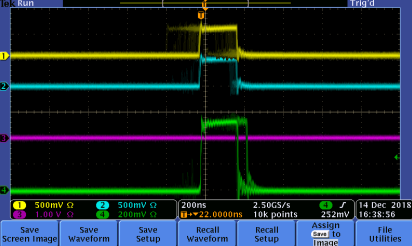
\includegraphics[width=\textwidth]{5Prototypes/53FinalPrototypes/531TritiumAveiro/Event_accepted_Aveiro_prototype.png}  
    \caption{Event accepted by the electronic system.\label{subfig:TrueTritiumEvent}}
    \end{subfigure}
    \hfill
    \begin{subfigure}[b]{0.42\textwidth}
    \centering
    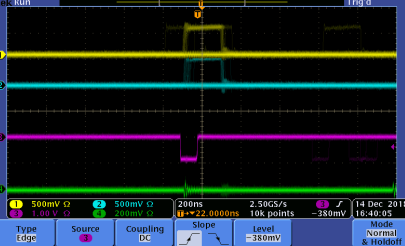
\includegraphics[width=\textwidth]{5Prototypes/53FinalPrototypes/531TritiumAveiro/Event_rejected_Aveiro_prototype.png}  
    \caption{Event rejected by the electronic system.\label{subfig:FalseTritiumEvent}}
    \end{subfigure}
 \caption{Two different situations of the electronic chain response. A.- Event accepted since veto has not detected it. B.- Event rejected since veto has detected it}
 \label{fig:ScreenshotElectronic}
\end{figure}


As can be seen, in Figure \ref{subfig:TrueTritiumEvent} both PMTs of the prototype have detect a time coincident event, which has not been detected for the veto, so this event is counted. In Figure \ref{subfig:FalseTritiumEvent}, a time coincidence event has been observed in the three PMTs, which means that it is a cosmic event, so this event is not counted.
\end{enumerate}